\documentclass[10pt,a4paper]{article}

\usepackage[T1]{fontenc}
\usepackage[utf8]{inputenc}
\usepackage[sc]{mathpazo}
\renewcommand{\ttdefault}{lmtt}
\linespread{1.06}
\usepackage[a4paper,margin=2.15cm,top=2.0cm,bottom=2.3cm]{geometry}
\usepackage{microtype}
\usepackage{amsmath,amssymb,mathtools}
\usepackage{graphicx}
\usepackage{booktabs}
\usepackage[font=small,labelfont=bf,skip=3pt]{caption}
\usepackage[round,authoryear]{natbib}
\usepackage{xcolor}
\usepackage[hidelinks]{hyperref}
\hypersetup{pdftitle={Hedging Bitcoin with Its Own Fear Gauge},pdfauthor={Gregor Albiez},pdfsubject={BTC volatility forecasting and BVIV hedging with a 15-minute VWAP ratchet},pdfkeywords={Bitcoin, implied volatility, BVIV, VWAP, hedging, HAR}}
\usepackage{enumitem}
\usepackage{titlesec}
\usepackage{url}
\usepackage{multicol}

\definecolor{ink}{HTML}{0b0b0b}
\titleformat{\section}{\normalfont\large\bfseries}{\thesection}{0.6em}{}
\titleformat{\subsection}{\normalfont\normalsize\bfseries}{\thesubsection}{0.6em}{}
\titlespacing*{\section}{0pt}{8pt plus 2pt minus 2pt}{3pt plus 1pt}
\titlespacing*{\subsection}{0pt}{6pt plus 2pt minus 1pt}{3pt plus 1pt}
\setlist{nosep,leftmargin=1.3em}
\setlength{\parskip}{0pt}
\widowpenalty=10000\clubpenalty=10000
\setlength{\textfloatsep}{8pt plus 2pt minus 2pt}
\setlength{\floatsep}{8pt plus 2pt minus 2pt}
\setlength{\intextsep}{8pt plus 2pt minus 2pt}
\renewcommand{\topfraction}{0.9}\renewcommand{\bottomfraction}{0.6}\renewcommand{\textfraction}{0.08}
\renewcommand{\floatpagefraction}{0.8}\setcounter{topnumber}{3}\setcounter{bottomnumber}{2}\setcounter{totalnumber}{5}
\setlength{\bibsep}{0.6pt}
\renewcommand{\bibfont}{\scriptsize}

\newcommand{\E}{\mathbb{E}}
\newcommand{\BVIV}{\textsc{bviv}}
\newcommand{\IV}{\mathit{IV}}
\newcommand{\RV}{\mathit{RV}}

% generated by scripts/run_paper.py -- do not edit
\newcommand{\NTest}{200}
\newcommand{\NTrain}{48}
\newcommand{\NRules}{87}
\newcommand{\SimDays}{900}
\newcommand{\EsRedAlways}{4.2}
\newcommand{\EsRedRatchet}{5.0}
\newcommand{\EsRedSwitch}{2.8}
\newcommand{\EsRedOracle}{2.3}
\newcommand{\VarRedAlways}{4.1}
\newcommand{\VarRedRatchet}{3.8}
\newcommand{\TailAlways}{5.9}
\newcommand{\TailRatchet}{7.9}
\newcommand{\CostAlways}{0.88}
\newcommand{\CostRatchet}{1.21}
\newcommand{\CostSwitch}{4.32}
\newcommand{\TurnSwitch}{24.6}
\newcommand{\TurnAlways}{0.9}
\newcommand{\TurnRatchet}{1.4}
\newcommand{\NotionalAlways}{7.0}
\newcommand{\NotionalRatchet}{9.6}
\newcommand{\DEsRatchet}{+0.61}
\newcommand{\DEsRatchetLo}{+0.41}
\newcommand{\DEsRatchetHi}{+0.81}
\newcommand{\ShareRatchet}{67}
\newcommand{\DEsSwitch}{\ensuremath{-}1.67}
\newcommand{\DMddRatchet}{\ensuremath{-}0.09}
\newcommand{\EsRedAlwaysTwo}{4.5}
\newcommand{\EsRedAlwaysThree}{1.8}
\newcommand{\EsRedAlwaysOnehalf}{4.9}
\newcommand{\CostAlwaysOnehalf}{1.32}
\newcommand{\VarRedAlwaysOnehalf}{3.1}
\newcommand{\VarRedSwitch}{1.9}
\newcommand{\DVarRatchet}{\ensuremath{-}0.48}
\newcommand{\DTailRatchet}{+2.1}
\newcommand{\ShareTailRatchet}{96}
\newcommand{\DEsSwitchLo}{\ensuremath{-}2.00}
\newcommand{\DEsSwitchHi}{\ensuremath{-}1.36}
\newcommand{\DEsFc}{+0.04}
\newcommand{\DEsFcLo}{\ensuremath{-}0.09}
\newcommand{\DEsFcHi}{+0.17}
\newcommand{\ShareAboveLadder}{47}
\newcommand{\NRatchetGrid}{72}
\newcommand{\DiagBaseAlways}{+0.28}
\newcommand{\DiagBaseRatchet}{+0.17}
\newcommand{\DiagClusterAlways}{+0.16}
\newcommand{\DiagClusterRatchet}{\ensuremath{-}0.09}
\newcommand{\RatchetZ}{\ensuremath{-}1}
\newcommand{\RatchetHl}{4}
\newcommand{\RatchetFloor}{1}
\newcommand{\RatchetFc}{with}
\newcommand{\SwitchZ}{\ensuremath{-}1}
\newcommand{\SwitchExit}{0.5}
\newcommand{\QlHarIvOne}{0.99}
\newcommand{\QlIvOne}{1.18}
\newcommand{\QlIvThirty}{0.81}
\newcommand{\QlHarIvThirty}{0.90}
\newcommand{\QlGarchOne}{1.26}
\newcommand{\QlIvrawThirty}{0.90}
\newcommand{\QlHarIvSeven}{0.89}
\newcommand{\QlIvSeven}{0.90}
\newcommand{\DmWinHarIvOne}{22}
\newcommand{\DmLossHarIvOne}{10}
\newcommand{\DmWinIvThirty}{34}
\newcommand{\DmLossIvThirty}{0}
\newcommand{\CorrDaily}{\ensuremath{-}0.21}
\newcommand{\CorrDown}{\ensuremath{-}0.26}
\newcommand{\CorrUp}{0.03}
\newcommand{\Vrp}{7.6}
\newcommand{\HedgeCarry}{6}
\newcommand{\Fee}{6}
\newcommand{\Slip}{10}
\newcommand{\EsRedPlacebo}{5.0}
\newcommand{\DEsPlacebo}{+0.02}
\newcommand{\DEsPlaceboLo}{\ensuremath{-}0.04}
\newcommand{\DEsPlaceboHi}{+0.07}
\newcommand{\SharePlacebo}{57}
\newcommand{\NPlacebo}{5}
\newcommand{\PgridN}{72}
\newcommand{\PgridMean}{+0.30}
\newcommand{\PgridMin}{\ensuremath{-}0.15}
\newcommand{\PgridMax}{+1.36}
\newcommand{\PgridSigPos}{29}
\newcommand{\PgridSigNeg}{0}
\newcommand{\PgridPaths}{64}
\newcommand{\PgridShifts}{3}
\newcommand{\PgridFloorZero}{+0.69}
\newcommand{\PgridFloorHalf}{+0.20}
\newcommand{\PgridFloorOne}{\ensuremath{-}0.00}
\newcommand{\PgridEsFloorZero}{3.5}
\newcommand{\PgridEsFloorOne}{4.9}
\newcommand{\PgridBestEs}{4.1}
\newcommand{\PgridBestCost}{4.2}
\newcommand{\PgridCorr}{\ensuremath{-}0.43}
\newcommand{\PgridAlwaysEs}{4.6}
\newcommand{\RobBaseline}{+0.61}
\newcommand{\RobLoBaseline}{+0.29}
\newcommand{\RobHiBaseline}{+0.91}
\newcommand{\RobTradingCostsDouble}{+0.59}
\newcommand{\RobLoTradingCostsDouble}{+0.27}
\newcommand{\RobHiTradingCostsDouble}{+0.89}
\newcommand{\RobTradingCostsHalf}{+0.62}
\newcommand{\RobLoTradingCostsHalf}{+0.30}
\newcommand{\RobHiTradingCostsHalf}{+0.92}
\newcommand{\RobFundingCarryZero}{+0.62}
\newcommand{\RobLoFundingCarryZero}{+0.30}
\newcommand{\RobHiFundingCarryZero}{+0.92}
\newcommand{\RobFundingCarryTwelve}{+0.60}
\newcommand{\RobLoFundingCarryTwelve}{+0.28}
\newcommand{\RobHiFundingCarryTwelve}{+0.90}
\newcommand{\RobVixLikeSpotVol}{+0.66}
\newcommand{\RobLoVixLikeSpotVol}{+0.37}
\newcommand{\RobHiVixLikeSpotVol}{+0.93}
\newcommand{\RobInverseLeverage}{+0.15}
\newcommand{\RobLoInverseLeverage}{\ensuremath{-}0.08}
\newcommand{\RobHiInverseLeverage}{+0.40}
\newcommand{\RobCrashesClusterInStress}{+0.29}
\newcommand{\RobLoCrashesClusterInStress}{\ensuremath{-}0.08}
\newcommand{\RobHiCrashesClusterInStress}{+0.66}
\newcommand{\RobSessionAnchoredVwap}{+0.62}
\newcommand{\RobLoSessionAnchoredVwap}{+0.30}
\newcommand{\RobHiSessionAnchoredVwap}{+0.92}
\newcommand{\RobPerpetualBtcBook}{+0.59}
\newcommand{\RobLoPerpetualBtcBook}{+0.28}
\newcommand{\RobHiPerpetualBtcBook}{+0.89}


\title{\vspace{-0.6em}\textbf{Hedging Bitcoin with Its Own Fear Gauge}\\[2pt]
\large Evidence from the BVIV Perpetual on Volatility Forecasts, Funding Costs and 15-Minute VWAP Timing}
\author{Gregor Albiez}
\date{October 2026}

\begin{document}
\maketitle
\vspace{-1.2em}

\begin{abstract}
\noindent A perpetual future on the Volmex \BVIV{} index of Bitcoin implied volatility has traded on Bitfinex since April 2024. We use 15-minute data from \LiveStart{} to \LiveEnd{}, including the perpetual's complete Bitfinex record, to ask how BTC volatility should be forecast when a 30-day implied index is observable, and whether a long-\BVIV{} position, possibly timed by a volume-weighted average price (VWAP) signal on 15-minute bars, hedges BTC. HAR augmented with implied variance is the best one-day forecast, significantly better than HAR; HAR-IV leads at a week and the bias-corrected index at a month, neither significantly. With rules frozen on simulated training data and executed one bar after the signal at the mark, a minimum-variance \BVIV{} hedge reduced the expected shortfall (ES) of a long-BTC book by \LiveEsAlways\% (95\% block-bootstrap CI \LiveEsAlwaysLo--\LiveEsAlwaysHi\%), mostly on a handful of crash days in 2026. Funding settled at its $\pm$0.25\% cap in \LiveFundCapShare\% of 8-hour periods and cost a permanently long contract \LiveFundAnnualPts{} vol points a year; the perpetual traded a median \$\LiveMedianUsd{} a day, and on its best days the hedge of a single bitcoin exceeded the market's open interest. A VWAP ratchet added \LiveDRatchet{} points of ES reduction (CI \LiveDRatchetCi), but placebos with the same triggers at shifted dates captured most of it: the gain is mainly extra downside exposure, which holding the ratchet's overlay permanently delivers too, with timing worth \LiveTiming{} points. A calibrated simulation with an arbitrage-free perpetual reproduces the forecast ranking and the split between exposure and timing. \BVIV{} perpetuals worked as a crash hedge, but funding, execution speed and capacity, not signal design, decide what that hedge is worth.
\end{abstract}

\section{Introduction}\label{sec:intro}

A holder of bitcoin, in spot or through a perpetual swap, faces two kinds of risk: an ordinary random walk, and sudden crashes in which liquidity disappears and implied volatility spikes. Futures hedges remove the first and, with it, the position itself; crash protection has required options. The Volmex \BVIV{} index measures 30-day BTC implied volatility in a model-free way \citep{volmex2024iv}, and it has traded as a USDT-margined perpetual on Bitfinex since April 2024 \citep{coindesk2024bitfinex}, on gTrade since June 2025 \citep{coindesk2025gtrade} and on Hyperliquid since September 2026 \citep{coindesk2026hyperliquid}. CME announced Bitcoin Volatility futures in May 2026 \citep{cme2026bvi}.

Whether long volatility hedges long BTC depends on the spot-vol correlation, which in BTC is weak and unstable. Positive return shocks have historically raised volatility more than negative ones \citep{bouri2017return,baur2018asymmetric}, an asymmetry that has faded \citep{takaishi2021time}; the BTC--DVOL correlation flipped positive in early 2023 \citep{coindesk2023dvol}, while \BVIV{} trended down through the 2024--25 rally \citep{coindesk2025rally}. Equity investors learned that long-volatility hedges look good \emph{ex ante} but are eroded by carry and costs \citep{whaley2013trading,alexander2016diversification,israelov2019pathetic}, except in genuine crises \citep{szado2009vix}. This raises two questions: what does such a hedge cost on a real crypto venue, and can it be \emph{timed} by a signal every intraday trader watches, price relative to its VWAP?

\paragraph{Contributions.} (i) We provide, to our knowledge, the first evidence on hedging BTC with a tradable implied-volatility perpetual, including an exact reconstruction of its funding rule, its realised costs and its capacity. (ii) We compare seven forecasts of BTC realised volatility, three of which use the official \BVIV{} index. (iii) We test VWAP timing with rules frozen on simulated data, single-path block-bootstrap inference and a \emph{timing placebo} that splits a rule's edge into exposure and timing. (iv) A calibrated simulation with an arbitrage-free perpetual serves as a controlled experiment. A pipeline regenerates every number from public data, except one dated order-book snapshot.

\section{The BVIV index and its perpetual}\label{sec:background}

\paragraph{Index.} \BVIV{} is a 30-day constant-maturity implied-volatility index that Volmex describes as model-free \citep{volmex2024iv}; secondary sources list Deribit and OKX options as inputs, and Volmex serves it at 15-minute resolution. Deribit's DVOL applies a VIX-style variance-swap calculation \citep{demeterfi1999guide} to Deribit options alone \citep{deribit2021dvol}. Implied variance exceeds subsequent realised variance on average: \citet{almeida2024risk} estimate about 0.14 a year in variance units for 2017--22, consistent with \citet{alexander2021bitcoin} and the equity evidence of \citet{carr2009variance}.

\paragraph{The Bitfinex perpetual.} One contract pays one dollar (USDt) per index point; the mark price is the index converted at USD/USDt and deviates from the official Volmex index by at most \LiveMarkGap\% on 95\% of 15-minute bars. Funding settles every eight hours. The status feed exposes the accrued premium $a$ of the perpetual over its mark, and the settled rates follow $\mathrm{sign}(a)\min\{\max(|a|-0.05\%,0),0.25\%\}$ exactly (largest deviation \LiveFitMax{} bp over all \LiveFundN{} settlements). The cap, 0.75\% of notional a day, binds often: in \LiveFundCapShare\% of settlements from April 2024 to October 2026, and longs paid on \LiveFundPosShare\%. A permanently long contract paid \LiveFundAnnualPts{} vol points a year on average (\LiveFundAnnualPct\% of notional), but the burden swung from \LiveFundPtsA{} points in 2024 and \LiveFundPtsB{} in 2025 to \LiveFundPtsC{} in 2026, when longs \emph{received} funding (Figure~\ref{fig:livemarket}). The market is tiny. The perpetual traded on \LiveDaysTraded{} of \LivePerpDays{} days, with a median daily volume of \$\LiveMedianUsd{} (mean \$\LiveMeanUsd), and only \LiveBarsTraded\% of 15-minute bars saw a trade. Its quoted mid sat a median \LivePremiumMedian\% above the mark, but dust orders at the top of the book put it more than 5\% away on \LiveMidWild\% of bars (up to +\LiveMidMax\%), so it is not an executable price.

\begin{figure}[t]
\centering
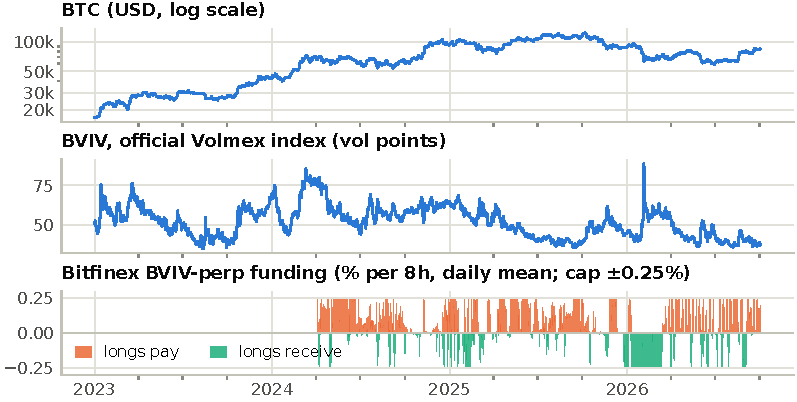
\includegraphics[width=\linewidth]{figures/live_market}
\caption{Live data, \LiveStart{} to \LiveEnd{}. Top: BTC (Binance). Middle: the official Volmex \BVIV{} index. Bottom: Bitfinex \BVIV{}-perpetual funding per 8-hour period (daily mean), paid by longs when positive.}
\label{fig:livemarket}
\end{figure}

\section{Data and volatility forecasts}\label{sec:data}

\paragraph{Data.} BTC is the Binance BTCUSDT spot market on 15-minute bars (\LiveDays{} days); quote volume over base volume gives each bar's exact VWAP. \BVIV{} is the official Volmex series from its public 15-minute history. The perpetual's marks, quotes, open interest and accrued funding come from about 1.3 million Bitfinex status snapshots (one a minute), which also yield every funding settlement; trades come from Bitfinex's trade candles. Table~\ref{tab:livefacts} summarises the sample. Volatility averaged \LiveRv\% against a mean index of \LiveIv{} (daily closes \LiveIvMin--\LiveIvMax); implied exceeded subsequent realised volatility on \LiveIvAbove\% of days. The daily spot-vol correlation was \LiveCorrDaily{} overall but moved from \LiveCorrA{} in 2023 through \LiveCorrB{} and \LiveCorrC{} to \LiveCorrD{} in 2026: the market became VIX-like. The index lags BTC: its 15-minute changes are autocorrelated (\LiveAc), and \LiveLagShare\% of its response to a 15-minute BTC return arrives in the three following bars, which matters for execution (Section~\ref{sec:hedge}).

\begin{table}[t]
\centering\small
\begin{tabular}{@{}lrrrrrr@{}}
\toprule
Moment & Live & 2023 & 2024 & 2025 & 2026 & Sim. \\
\midrule
Realised vol, annualised (\%) & 46.6 & 43.2 & 53.0 & 44.6 & 44.3 & 51.5 \\
Mean BVIV (vol pts) & 51.9 & 52.4 & 60.2 & 48.3 & 45.2 & 57.1 \\
IV $-$ subsequent 30d RV (vol pts) & 6.8 &  &  &  &  & 7.6 \\
Share of days IV $>$ RV (\%) & 75 &  &  &  &  & 78 \\
corr(daily return, $\Delta$IV) & \ensuremath{-}0.10 & 0.32 & 0.03 & \ensuremath{-}0.30 & \ensuremath{-}0.59 & \ensuremath{-}0.21 \\
corr on falling 15m bars & \ensuremath{-}0.24 &  &  &  &  & \ensuremath{-}0.26 \\
corr on rising 15m bars & 0.03 &  &  &  &  & 0.03 \\
AC(1) of 15m index changes & 0.20 &  &  &  &  & -- \\
Excess kurtosis, daily returns & 3.4 &  &  &  &  & 3.7 \\
Worst daily log return ($-$\%) & 15.1 &  &  &  &  & 15.0 \\
\bottomrule
\end{tabular}

\caption{Stylised facts: live sample (\LiveStart{} to \LiveEnd) and by calendar year, against the median of the simulation's \NTest{} test paths (Section~\ref{sec:sim}).}
\label{tab:livefacts}
\end{table}

\paragraph{Forecasts.} From 15-minute log returns we compute daily realised variance \citep{andersen2003modeling}; fifteen minutes is coarser than the 5-minute rule of thumb \citep{liu2015does} but matches the hedge's frequency. Each model forecasts the average daily variance over the next $h\in\{1,7,30\}$ days from information at day $t$'s close: a random walk, RiskMetrics EWMA \citep{jpmorgan1996riskmetrics}, GARCH(1,1) with Student-$t$ errors re-estimated monthly, the heterogeneous autoregressive (HAR) model of \citet{corsi2009simple} with a 7-day week, the index itself, raw ($\IV_t^2/365$, ``IV-raw'') and bias-corrected (``IV''), and HAR augmented with implied variance:
\begin{equation}\label{eq:har}
\ln\overline{\RV}_{t+1:t+h}=\beta_0+\beta_d\ln\RV_t+\beta_w\ln\overline{\RV}_{t-6:t}+\beta_m\ln\overline{\RV}_{t-29:t}+\beta_{iv}\ln(\IV_t^2/365)+\varepsilon_{t+h}.
\end{equation}
HAR and IV are the special cases without the implied or the realised terms. Regressions run in logs, so forecasts $\exp(\hat y+s^2/2)$, with $s^2$ the residual variance, are positive, and are re-estimated daily on an expanding window of targets already observed. We evaluate the \LiveForecastN{} one-day forecasts from 2024 on with QLIKE, which is robust to proxy noise \citep{patton2011volatility}, the Mincer--Zarnowitz $R^2$ and Diebold--Mariano (DM) tests against HAR with Newey--West variance \citep{mincer1969evaluation,diebold1995comparing}.

\begin{table}[t]
\centering\small
\begin{tabular}{@{}lrrrrrrrrr@{}}
\toprule
 & \multicolumn{3}{c}{$h=1$ day} & \multicolumn{3}{c}{$h=7$ days} & \multicolumn{3}{c}{$h=30$ days} \\
\cmidrule(lr){2-4} \cmidrule(lr){5-7} \cmidrule(lr){8-10}
Model & QL ratio & MZ $R^2$ & DM $t$ & QL ratio & MZ $R^2$ & DM $t$ & QL ratio & MZ $R^2$ & DM $t$ \\
\midrule
RW & 1.71 & 0.16 & 10.47 & 1.33 & 0.15 & 2.56 & 1.42 & 0.09 & 1.70 \\
EWMA & 1.27 & 0.09 & 5.18 & 1.40 & 0.10 & 2.91 & 1.87 & 0.09 & 2.53 \\
GARCH & 1.41 & 0.10 & 8.96 & 1.95 & 0.09 & 5.29 & 3.52 & 0.14 & 3.21 \\
HAR & 1.00 & 0.21 & -- & 1.00 & 0.19 & -- & 1.00 & 0.02 & -- \\
IV-raw & 1.24 & 0.15 & 6.07 & 1.06 & 0.22 & 0.79 & 0.91 & 0.26 & \ensuremath{-}0.65 \\
IV & 1.17 & 0.15 & 2.72 & 1.02 & 0.20 & 0.15 & \textbf{0.84} & 0.18 & \ensuremath{-}1.54 \\
HAR-IV & \textbf{0.96} & 0.26 & \ensuremath{-}2.25 & \textbf{0.95} & 0.25 & \ensuremath{-}0.74 & 0.92 & 0.16 & \ensuremath{-}0.60 \\
\bottomrule
\end{tabular}

\caption{Live out-of-sample forecast accuracy, 2024 to October 2026. QL ratio: a model's QLIKE over HAR's (best in bold). DM $t$: Diebold--Mariano statistic against HAR (negative favours the model).}
\label{tab:liveforecast}
\end{table}

\paragraph{Results.} Table~\ref{tab:liveforecast} confirms the pattern documented on Deribit data by \citet{hoang2020forecasting}. At one day HAR-IV is best (QLIKE ratio \LiveQlOne) and significantly better than HAR (DM \LiveDmOne), while the index alone is worse (\LiveQlIvOne) and GARCH on daily returns lags (\LiveQlGarchOne), as \citet{bergsli2022forecasting} found for BTC. At longer horizons the leading models (HAR, HAR-IV and the index) are not significantly different. HAR-IV stays ahead at seven days (\LiveQlSeven; DM \LiveDmSeven), where the bias-corrected index is no better than HAR (\LiveQlIvSeven); at 30 days the bias-corrected index is best (\LiveQlThirty; DM \LiveDmThirty), followed by raw IV (\LiveQlRawThirty) and HAR-IV (\LiveQlHarThirty). The calibrated simulation has the same winner at every horizon (Section~\ref{sec:sim}).

\section{Hedging framework}\label{sec:hedge}

\paragraph{P\&L.} The book is long $q$ BTC at price $S_t$ and long $H_t\ge0$ \BVIV{}-perpetual contracts with mark $F_t$. A position $H_t$ held from the close of 15-minute bar $t$ earns over bar $t{+}1$
\begin{equation}\label{eq:pnl}
\begin{split}
\Pi_{t+1}={}&q\,(S_{t+1}-S_t)-\mathbb{1}_{\text{perp}}\,q\,S_t f_t\,\Delta t+H_t\,(F_{t+1}-F_t)-H_t\,\psi_t\\
&-(H_{t+1}-H_t)(P_{t+1}-F_{t+1})-c\,|H_{t+1}-H_t|\,F_{t+1},
\end{split}
\end{equation}
where $\mathbb{1}_{\text{perp}}=1$ for a perpetual BTC book, $\Delta t$ is the bar length in years, $f_t$ the BTC perpetual's annualised funding rate, $\psi_t$ the \BVIV{} funding per contract, booked on the position held at each settlement, $P_t$ the fill price, and $c$ a proportional cost of \Fee{} bp fee plus \Slip{} bp slippage per side. On live data $\psi_t$ is the settled funding. A perpetual on an index $I_t$ is priced at the expected index sampled at a random time \citep{he2022perpetual,ackerer2025perpetual}; in the simulation we split its funding into an arbitrage-free drift transfer $\E_t[I_{t+1}]-I_t$ and a carry premium.

\paragraph{Execution.} On live data a decision at the close of bar $t$ is executed at the close of bar $t{+}1$ at the mark ($P=F$), plus costs. Same-bar execution would collect the index's predictable catch-up after a BTC move (Section~\ref{sec:data}), and the quoted mid is not executable (Section~\ref{sec:background}); both are sensitivities (quotes capped at $\pm$5\% of the mark), as are costs of 50 bp per side on top of the fee, the price impact of one bitcoin's hedge in the order book a day after the sample. No position is held before the listing at 09:00 UTC on 3 April 2024.

\paragraph{Hedge ratios and signal.} The minimum-variance hedge is $H_t^\ast=-qS_t\beta_t$, with $\beta_t=\mathrm{Cov}_t(r,\Delta F)/\mathrm{Var}_t(\Delta F)$ estimated on 15-minute BTC log returns $r$ and mark changes $\Delta F$ by an EWMA (half-life 14 days) \citep{johnson1960theory,ederington1979hedging}; we impose $H\ge0$. A downside ratio $\beta^-_t=\E_t[r\,\Delta F\mid r<0]/\E_t[\Delta F^2\mid r<0]$ on falling bars, shrunk towards $\beta_t$ with a two-day prior, gives the crash hedge $H^-_t$. The breakdown statistic compares the price with its rolling 24-hour VWAP,
\begin{equation}\label{eq:z}
z_t=\ln\!\big(S_t/\mathrm{VWAP}^{24h}_t\big)\big/\big(\hat\sigma_t\sqrt{1/3}\big),
\end{equation}
because for Brownian prices the gap between the last price and its average over a window $w$ has standard deviation $\sigma\sqrt{w/3}$. Here $\hat\sigma_t$ is the daily volatility implied by a causal EWMA (half-life one day) of 15-minute squared returns, de-seasonalised by a trailing hour-of-week profile \citep{andersen1997intraday,hansen2024periodicity}.

\paragraph{Rules.} All rules are long-only, their targets are capped at 50\% of BTC notional, and they trade only when the target leaves a 25\% band around the position \citep{whalley1997asymptotic}, so held positions can drift above the cap (on live data at most \LiveMaxNotional\% for the minimum-variance hedge and \LiveMaxNotionalHalf\% for 1.5$\times$). \emph{Always-on} holds $\lambda H^\ast_t$ with $\lambda\in\{1,1.5\}$. The \emph{VWAP-switch} holds $H^-_t$ while a gate is on, switching on at $z_t<z_{in}$ and off at $z_t>z_{out}$, for at least four hours. The \emph{VWAP-ratchet} holds a core $\varphi H^\ast_t$ plus an overlay $o_t$ that jumps to 1 on a breakdown and decays with half-life $\tau$:
\begin{equation}\label{eq:ratchet}
o_t=\begin{cases}1 & z_t<z_{in}\\ 2^{-1/(96\tau)}\,o_{t-1} & \text{otherwise,}\end{cases}\qquad
H_t=\varphi H_t^\ast+o_t\max\!\big(H^-_t\,m_t-\varphi H_t^\ast,\,0\big),
\end{equation}
where $m_t=\min\{\max(e^{\kappa_t},0.5),1.5\}$ optionally scales the overlay by forecast ``cheapness'' $\kappa_t$: the log ratio of the 30-day HAR-IV forecast to implied variance, less its trailing 180-day median, lagged one day.

\paragraph{Protocol.} Rule parameters were selected on \NTrain{} simulated training paths (Section~\ref{sec:sim}), out of 72 ratchets and six switches, by median ES reduction net of costs, before the live pipeline was written. The selected ratchet keeps the full core ($\varphi=\RatchetFloor$), triggers at $z<\RatchetZ$, decays with a half-life of \RatchetHl{} days and uses forecast sizing; the selected switch enters at $z<\SwitchZ$ and exits at $z>\SwitchExit$. The live sample is therefore out of sample for the rules, which avoids data snooping \citep{white2000reality,hansen2005spa,bailey2014pseudo}, although the simulator's calibration targets include coarse features of the 2023--26 market. Signals warm up on 2023 data, and hedging is evaluated over the \LiveEvalDays{} days since the listing, \LiveEvalStart{} to \LiveEvalEnd. On a single path we report 95\% intervals from a paired stationary block bootstrap over days (mean block ten days, 2{,}000 draws); for mean blocks of 1, 2, 5, 10, 20, 30 and 40 days the lower bound of the always-on ES reduction lies between \LiveBlockLoMin\% and \LiveBlockLoMax\%. The timing placebo shifts a ratchet's trigger series circularly within the whole weeks of the evaluation window, by every multiple of a week for the selected rule (\LivePlaceboN{} shifts) and of two weeks for each rule of the grid (\LiveGridShifts{} shifts). It keeps the triggers' number, clustering and hour-of-week profile but breaks their link to the market. A ratchet's edge over the always-on hedge then splits into \emph{exposure}, the placebo mean minus the always-on result, and \emph{timing}, the ratchet minus its placebo mean.

\section{Results on live data}\label{sec:live}

\begin{table}[t]
\centering\small\setlength{\tabcolsep}{4.5pt}
\begin{tabular}{@{}lrrrrrrrrr@{}}
\toprule
Rule & ES red. & Var red. & Max DD & Tail offset & Hedge P\&L & Funding & Trading & Turnover & Notional \\
\midrule
Unhedged & 0.0 & 0.0 & 53.0 & 0.0 & 0.00 & 0.00 & 0.00 & 0.0 & 0.0 \\
Always-on (MV) & 17.9 & 14.9 & 41.7 & 26.9 & 2.13 & 1.41 & 0.20 & 1.3 & 11.1 \\
Always-on, 1.5$\times$ & 20.1 & 13.2 & 41.9 & 38.7 & 1.07 & 2.21 & 0.29 & 1.8 & 16.7 \\
VWAP-switch & 18.8 & 12.6 & 42.5 & 25.6 & 6.70 & \ensuremath{-}0.26 & 5.17 & 32.3 & 4.6 \\
VWAP-ratchet & 20.3 & 15.0 & 42.6 & 30.6 & 1.34 & 2.67 & 0.37 & 2.3 & 12.5 \\
\bottomrule
\end{tabular}

\caption{Hedging a 1-BTC spot book with the Bitfinex \BVIV{} perpetual, \LiveEvalStart{} to \LiveEvalEnd{}, executed one bar after the signal at the mark (\%, except turnover). ES/Var red.: reduction in daily ES$_{97.5}$ and variance against unhedged. Max DD: maximum drawdown. Tail offset: hedge P\&L net of costs as a share of BTC losses on the worst 5\% of days. Hedge P\&L (index P\&L minus funding), Funding and Trading (fees and slippage): \% of BTC notional a year. Turnover: perpetual notional traded per year over BTC notional. Notional: average hedge notional in \% of BTC.}
\label{tab:livehedge}
\end{table}

\begin{figure}[t]
\centering
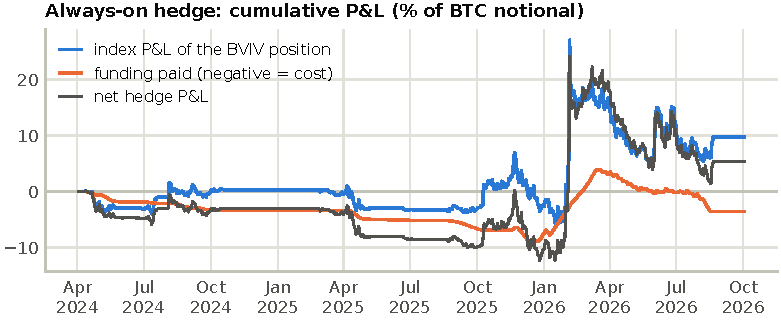
\includegraphics[width=\linewidth]{figures/live_hedge}
\caption{Always-on minimum-variance hedge on live data: cumulative index P\&L of the \BVIV{} position, cumulative funding (negative = paid), and hedge P\&L net of funding, in \% of BTC notional.}
\label{fig:livehedge}
\end{figure}

\paragraph{The hedge works, in crashes.} The minimum-variance hedge reduced ES by \LiveEsAlways\% (block-bootstrap CI \LiveEsAlwaysLo--\LiveEsAlwaysHi\%) and variance by \LiveVarAlways\% (\LiveVarAlwaysLo--\LiveVarAlwaysHi\%), and cut the maximum drawdown from \LiveMddUnhedged\% to \LiveMddAlways\% with an average notional of \LiveNotionalAlways\% of the BTC position (Table~\ref{tab:livehedge}). It was held on \LiveTimeOnAlways\% of bars and off whenever the estimated spot-vol covariance was positive, including on \LiveTailFlat{} of the \LiveTailDays{} days in the unhedged ES tail. Net of funding (Figure~\ref{fig:livehedge}), its P\&L summed to \LiveHedgeTotal\% of BTC notional: the ten best days contributed +\LiveTopTen\% of notional and all other days \LiveExTopTen\%. The ten worst BTC days cost the unhedged book \LiveWorstBtc\% of notional, and the hedge earned back \LiveWorstHedge\%, \LiveWorstShare\% of that loss. The ES reduction was \LiveEsYearA\% in 2024, \LiveEsYearB\% in 2025 and \LiveEsYearC\% in 2026; without the best day it is \LiveEsExBest\%, without the five best \LiveEsExFive\%. Over 7- and 14-day horizons it is \LiveEsWeek\% and \LiveEsFortnight\%, so the daily figure is not an artefact of the index lagging across day boundaries. Funding cost the hedge \LiveFundAlways\% of BTC notional a year: it paid \LiveFundHedgeA\% a year in 2024 and \LiveFundHedgeB\% in 2025 and received \LiveFundHedgeC\% in 2026.

\paragraph{The best day.} On \LiveBestDay{} the hedge returned \LiveBestDayPct\% of BTC notional while BTC fell by \LiveEpBtc\% (Figure~\ref{fig:liveepisode}). \BVIV{} stood at \LiveEpIvMidnight{} at midnight and \LiveEpIvBefore{} an hour before BTC broke below the ratchet's VWAP band on the bar ending \LiveEpTrigger{} UTC; it was \LiveEpIvTrigger{} on that bar, \LiveEpIvAfter{} by \LiveEpIvAfterTime{} and peaked at \LiveEpIvPeak{} at \LiveEpIvPeakTime. All rules entered the day with \LiveEpOpenMin--\LiveEpOpenMax{} contracts. As the index's 15-minute moves exploded, the EWMA hedge ratio fell and the rules sold into the spike, the always-on hedge to \LiveEpCloseAlways{} contracts by the close; the ratchet's overlay kept it up to \LiveEpRatchetMax\% larger.

\begin{figure}[t]
\centering
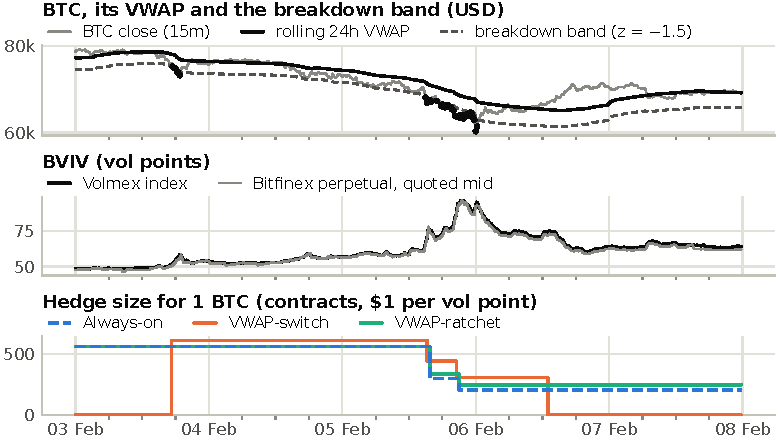
\includegraphics[width=\linewidth]{figures/live_episode}
\caption{The best hedge day, \LiveBestDay{}, and the days around it at 15-minute resolution (UTC, bar open times). Top: BTC, its rolling 24-hour VWAP and the ratchet's breakdown band (dots: $z_t<z_{in}$). Middle: the Volmex index and the Bitfinex perpetual's quoted mid. Bottom: hedge sizes of the three rules for a 1-BTC book.}
\label{fig:liveepisode}
\end{figure}

\begin{table}[t]
\centering\small
\begin{tabular}{@{}lrrrr@{}}
\toprule
Variant & Always-on & 1.5$\times$ & Switch & Ratchet \\
\midrule
Same-bar execution & 19.1 (+2.5) & 20.5 (+1.5) & 20.1 (+7.6) & 21.1 (+2.7) \\
Execution 1 hour later & 16.0 (+0.4) & 17.3 (\ensuremath{-}1.9) & 14.1 (\ensuremath{-}3.0) & 18.3 (\ensuremath{-}2.0) \\
Execution 1 day later & 12.6 (\ensuremath{-}1.4) & 11.2 (\ensuremath{-}5.3) & 10.3 (\ensuremath{-}4.3) & 13.2 (\ensuremath{-}3.0) \\
Fills at the quoted mid & 17.7 (+1.6) & 19.8 (+0.4) & 18.4 (+2.8) & 20.2 (+0.4) \\
Book costs (50 bp + fee) & 17.8 (+1.4) & 20.0 (+0.1) & 18.2 (\ensuremath{-}11.4) & 20.1 (+0.1) \\
No trading costs & 18.0 (+2.1) & 20.1 (+1.1) & 19.0 (+6.7) & 20.3 (+1.4) \\
Funding ignored & 17.9 (+3.3) & 20.0 (+3.0) & 18.7 (+1.3) & 20.3 (+3.6) \\
Perpetual BTC book & 18.0 (+1.9) & 20.1 (+0.8) & 18.9 (+1.5) & 20.3 (+1.0) \\
\bottomrule
\end{tabular}

\caption{Live-data sensitivities, frozen rules, one change at a time to the baseline (execution one bar after the signal at the mark, \Fee{}+\Slip{} bp per side): ES reduction in \% (hedge P\&L net of funding and trading costs, \% of BTC notional a year).}
\label{tab:livesens}
\end{table}

\paragraph{Timing adds little beyond exposure.} The switch traded \LiveTurnSwitch{} times the BTC notional a year; its ES reduction differed from the always-on hedge's by \LiveDSwitch{} points, not significantly (CI \LiveDSwitchCi), and at the book's prices it would have paid \LiveBookCostSwitch\% of notional a year in trading costs. The ratchet beat the always-on hedge by \LiveDRatchet{} points (CI \LiveDRatchetCi) and the 1.5$\times$ hedge by \LiveDRatchetHalf{} (CI \LiveDRatchetHalfCi). Its \LivePlaceboN{} placebos reduced ES by \LivePlaceboMean\% on average, 90\% of them between \LivePlaceboLo\% and \LivePlaceboHi\% (Figure~\ref{fig:livetiming}, left), so \LiveSize{} points of the edge are exposure and \LiveTiming{} timing; the ratchet beats \LivePlaceboBeaten\% of its placebos (\LiveSamePlacebo\% with same-bar fills, \LiveMidPlacebo\% at quoted mids). The exposure is more than notional: scaled to the placebos' notional (\LiveMatchedScale$\times$), the minimum-variance hedge reduces ES by \LiveMatchedEs\%, whereas the ratchet's overlay held permanently reduces it by \LiveHeldEs\%, more than any timed rule (at most \LiveGridMaxEs\%), for \LiveHeldCost\% of notional a year against the ratchet's \LiveRatchetCost\%. Across the 72-rule grid, timing adds \LiveGridZero{} points without a core hedge (rules beat a mean \LiveGridRankZero\% of their placebos), \LiveGridHalf{} with half a core and \LiveGridOne{} with the full core (\LiveGridRankOne\%; \LiveGridSigOne{} of \LiveGridNOne{} rules beat at least 95\%; right panel). VWAP breakdowns time protection far better than chance when nothing else is held, but they flag a sell-off already under way, and a core hedge captures most of their value.

\begin{figure}[t]
\centering
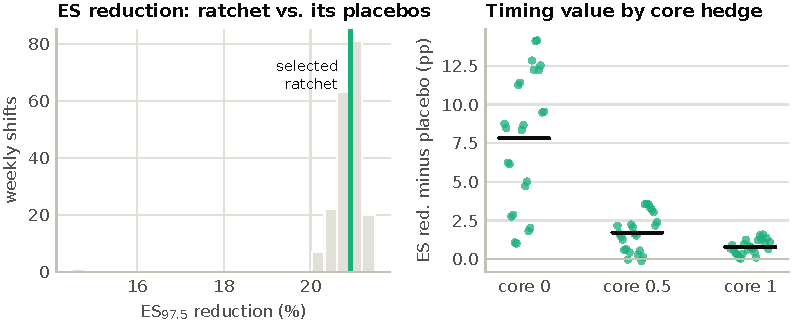
\includegraphics[width=\linewidth]{figures/live_timing}
\caption{Timing placebos on live data. Left: ES reduction of the selected ratchet (line) against its \LivePlaceboN{} weekly circular shifts of its triggers. Right: timing value of each of the 72 ratchet configurations (ES reduction minus the mean over \LiveGridShifts{} two-weekly shifts) by core size; bars mark the means.}
\label{fig:livetiming}
\end{figure}

\paragraph{Execution and capacity.} Costs, funding and fills at quoted mids barely move the ES reductions, which are dominated by crash days (Table~\ref{tab:livesens}). Speed matters most: same-bar execution would raise the always-on ES reduction to \LiveSameEsAlways\%, while executing one hour or one day late lowers it to \LiveDelayHour\% and \LiveDelayDay\%. Same-bar fills would also lift the switch's net hedge P\&L from \LiveNetSwitch\% to \LiveSameNetSwitch\% a year, by collecting the index's catch-up. Capacity binds. When held, the hedge of one bitcoin was a median \LiveContracts{} contracts, against a median open interest of \LiveMedianOi{} on those bars, and exceeded the whole open interest on \LiveAboveOi\% of those bars (\LiveAboveOiAll\% of all bars). On its five best days it was \LiveOiMultipleLo{} to \LiveOiMultipleHi{} times the open interest; on \LiveBestDay{} it traded \LiveBestTraded{} contracts while the market traded \LiveBestMarket, and \LiveDeadAlways\% of its trades fell on days without a single trade in the market. A book snapshot on \LiveBookDate{} shows market makers quoting size: buying or selling one bitcoin's hedge would have cost \LiveBookBuy\% and \LiveBookSell\% from the mid of the first levels with at least one contract, which were \LiveBookSizeSpread\% apart (the \LiveBookTopSpread\% top-of-book spread rested on a dust bid), and depth within 2.5\% of the mid would have held the hedge of about \LiveBookBtc{} bitcoins.

\section{The controlled experiment}\label{sec:sim}

One path cannot separate rules reliably, so we repeat the study in a simulated market calibrated to the stylised facts (Table~\ref{tab:livefacts}, last column). Log-variance is the sum of a slow and a fast Ornstein--Uhlenbeck factor; the fast factor tracks a three-state hidden regime (calm, stress, euphoria) and receives EGARCH-type shocks \citep{nelson1991conditional} whose signed loading on the return shock is $-0.30$\slash$-0.60$\slash$+0.25$ by regime; jumps cluster in stress, and volatility and volume are seasonal within the day and week. The index is the square root of the model's exact expectation of 30-day average variance (a Feynman--Kac product over regime paths), scaled by a variance premium and perturbed by persistent sentiment. The perpetual's funding is the exact one-bar drift transfer plus a carry of \HedgeCarry{} vol points a year, so it offers no free lunch from mean reversion; unit tests check both expectations against brute-force simulation. The simulated index has neither the live index's lag nor a funding cap, so the simulation does not speak to execution delay or the funding regime. Each path has \SimDays{} days; rules are selected on \NTrain{} training paths and evaluated on \NTest{} test paths.

\begin{table}[t]
\centering\small
\begin{tabular}{@{}lrrrrrrrr@{}}
\toprule
Rule & ES red. & Var red. & Max DD & Tail offset & Carry & Trading & Turnover & Time on \\
\midrule
Unhedged & 0.0 & 0.0 & 51.7 & 0.0 & 0.00 & 0.00 & 0.0 & 0 \\
Always-on (MV) & 3.3 & 3.2 & 52.0 & 4.7 & 0.58 & 0.14 & 0.9 & 93 \\
VWAP-switch & 2.2 & 1.2 & 53.1 & 4.2 & 0.31 & 3.21 & 20.0 & 34 \\
VWAP-ratchet & 3.5 & 2.5 & 51.5 & 6.8 & 0.80 & 0.19 & 1.2 & 98 \\
Oracle (infeasible) & 1.3 & 1.2 & 51.1 & 2.7 & 0.08 & 0.22 & 1.4 & 9 \\
\bottomrule
\end{tabular}

\caption{Simulation: hedging a long-BTC book on \NTest{} test paths (medians; \% unless stated). Columns as in Table~\ref{tab:livehedge}; Carry: funding carry paid (\% of BTC notional a year); Time on: share of bars hedged. Placebo timing: the selected ratchet with circularly shifted triggers (mean of \NPlacebo{} shifts).}
\label{tab:simhedge}
\end{table}

\paragraph{Findings.} The forecast ranking is the same as on live data: HAR-IV is best at one day (median QLIKE ratio \QlHarIvOne) and seven days (\QlHarIvSeven), the bias-corrected index at 30 days (\QlIvThirty). The hedging gains are smaller (Table~\ref{tab:simhedge}): the simulation has neither the 2026 crash cluster nor its strong spot-vol correlation (\LiveCorrD{} against \CorrDaily). The always-on hedge reduces ES by \EsRedAlways\%; unlike on live data, where the two cannot be told apart, the switch trails it by \DEsSwitchAbs{} points (CI [\DEsSwitchLo, \DEsSwitchHi]). The ratchet beats it by \DEsRatchet{} points (CI [\DEsRatchetLo, \DEsRatchetHi]) but its placebo by only \DEsPlacebo{}, and a 1.5$\times$ hedge reaches the same ES reduction (\EsRedAlwaysOnehalf\%): as on live data, the edge is mostly exposure. Across the grid (\PgridPaths{} paths, \PgridShifts{} shifts per rule), timing adds \PgridFloorZero{} points without a core and \PgridFloorOne{} with the full core. In \NRobust{} further paths with common random numbers, the ratchet's edge survives doubled or halved trading costs and a carry of 0 to 24 vol points a year (\RobCostMin{} to \RobCostMax{} points). It shrinks to \RobInverseLeverage{} points under inverse leverage and to \RobCrashesClusterInStress{} when crashes cluster in stress, where the CIs include zero.

\section{Limitations and conclusion}\label{sec:conclusion}

The live sample is one path of \LiveEvalDays{} days, and the hedge's gains rest on a few crashes in 2026 (without the five best hedge days the ES reduction falls from \LiveEsAlways\% to \LiveEsExFive\%), which the bootstrap quantifies but cannot remove. Fills one bar after the signal at the mark plus costs are a benchmark for small books, not a realisable P\&L at scale: on its best days the market's volume and open interest could not have absorbed even a 1-BTC hedge, and we observe the order book only once, after the sample. The gains also assume that the shorts stayed solvent through a \LiveEpRise\% intraday rise of the index and that USDt held its peg; we do not model margin, liquidation, auto-deleveraging or venue failure. Oracle risk \citep{hyperliquid2026funding} and algorithmic flow at the 15-minute boundary \citep{kim2026quarter} argue for working orders inside the bar by VWAP slicing \citep{berkowitz1988total,konishi2002optimal,bialkowski2008improving}.

Four lessons follow. (1)~HAR augmented with implied variance is the best one-day BTC volatility forecast; at a week HAR-IV and at a month the bias-corrected implied index lead HAR, but not significantly. (2)~A minimum-variance \BVIV{} hedge cut tail risk by \LiveEsAlways\% over 2024--26, mostly through a few crashes with spiking implied volatility in 2026. Holding beats switching on costs and in the simulation; on live data the two cannot be told apart. (3)~Its price is funding, which on Bitfinex is capped, volatile and usually paid by longs; its limits are execution speed and capacity. (4)~A 15-minute VWAP breakdown is real but secondary information: without a core hedge it beats random timing, but with one most of a ratchet's edge is extra exposure, which holding its overlay permanently delivers too; timing adds \LiveTiming{} points for the frozen rule and \LiveGridOne{} across the full-core grid, up to \LiveGridStrictHi\% of the edge for strict thresholds. Intraday timing rules should face such placebos before they earn their complexity.

\clearpage
\section*{References}
\renewcommand{\bibsection}{}
\setlength{\columnsep}{14pt}
\begin{multicols}{2}
\bibliographystyle{plainnat}
\bibliography{references}
\end{multicols}

\end{document}
